\documentclass[11pt,letterpaper]{article}

\usepackage{graphicx}
\usepackage[margin=1in]{geometry}
\usepackage{amsmath}
\usepackage[T1]{fontenc}
\usepackage[utf8]{inputenc}
\usepackage{authblk}
\usepackage{fancyhdr}
\usepackage{lastpage}
\usepackage[parfill]{parskip}
\usepackage{subcaption}

\pagestyle{fancyplain}

% Headers
\lhead{}
\chead{}
\rhead{}

% Footers
\lfoot{}
\cfoot{}
\rfoot{\footnotesize Page \thepage\ of \pageref{LastPage}}

\renewcommand{\headrulewidth}{0.0pt} % No header rule
\renewcommand{\footrulewidth}{0.4pt} % Thin footer rule

\title{Federated Consistency Simulation: \\
Effect of Topological Configuration on Eventual Consistency (Stentor)}
\date{August 22, 2016}
\author[ ]{Benjamin Bengfort}
\author[ ]{Pete Keleher}
\affil[ ]{Department of Computer Science}
\affil[ ]{University of Maryland}
\affil[ ]{\textit{\{bengfort,keleher\}@cs.umd.edu}}

\begin{document}

\maketitle

The results presented in this paper are a rerunning of the simulation topologies and configuration discussed in the August 10, 2016 results report (``Increasing Likelihood of Conflicts Across Many Objects'') but with two additional simulation topologies that extend Eventual consistency so as to show that Federated does not benefit solely from the spanning tree in the middle of the distributed network. Here we introduce a new type of eventually consistent replica server called ``Stentor'' that performs anti-entropy slightly differently than both the basic Eventual and Federated consistency implementations. These results also present the reworking of our eventual consistency model as anti-entropy with object vector gossiping.

The basic \textbf{Eventual} replica server performs anti-entropy with $n$ uniform randomly chosen neighbors (by default $n=1$) from anywhere in the topology at an interval specified by the tick parameter, $\frac {T} {4}$. It sends a \texttt{Gossip} message to the neighbor with an \textit{object version vector} of the latest version of every object in its log. On receipt of a \texttt{Gossip} message, eventual nodes will compare the sent versions of all objects with their local log; if the RPC versions have a later object version than what's currently in their log, they append the new version (latest writer wins), otherwise they send a \texttt{GossipResponse} message with locally greater versions back to the initiating node who amends its log accordingly.

\textbf{Federated Eventual} nodes have a slightly different mechanism as they must deal with the presence of strongly consistent nodes. For each anti-entropy interval, Federated Eventual nodes choose $n$ (by default $n=1$) anti-entropy partners according to two Bernoulli distributions: one that specifies the likelihood of ``synchronizing'' with a Raft node, $P_{sync}$ and one that specifies the likelihood of anti-entropy in the local area vs. across the wide area if not synchronizing, $P_{local}$. All of our Federated simulations to date have had probabilities set as follows: $P_{sync} = 0.3$, $P_{local}=0.6$. Note that in our simulation the all eventual topology consists of Federated Eventual nodes and therefore have a slight preference to choosing local nodes vs. remote nodes thanks to $P_{local}$.

\textbf{Stentor} nodes engage both the local and wide area for every anti-entropy session. Instead of choosing $n$ neighbors with uniform random probability at each anti-entropy session, they always select one node from the wide area and one node from the local area to conduct anti-entropy with. Both the local nodes and the wide area nodes are chosen with uniform random probability. We have created two Stentor-topologies: one that has a core of Stentor (``stentor'') nodes (similar to the core of Raft nodes) and one where all Replicas are Stentor nodes (``stentor-complete''). The purpose of the ``stentor'' simulation is to show that a local core of nodes that is always forwarding information across the wide area is not the primary benefit of a Federated system. The purpose of ``stentor-complete'' is to show the performance difference between ``stentor'' and a regular ``eventual'' system.

The simulation settings were fairly conservative in order to promote a quick simulation result, particularly with respect to latency. Most simulation settings are specified in Table \ref{table:settings}.

\begin{table}[!h]
\makebox[\textwidth][c]{
\centering
\begin{tabular}{|r|lllll|}
\hline
 Setting & Eventual & Federated & Stentor-Complete & Stentor & Raft \\
\hline
 Anti-Entropy Delay & 2500ms & 2500ms & 2500ms & 2500ms & N/A\\
 Election Timeout   & N/A & $U(10000, 20000)$ & N/A &  N/A & $U(10000, 20000)$ \\
 Heartbeat Interval & N/A & 5000ms & N/A &  N/A & 5000ms \\
 Aggregate Writes   & N/A & True & N/A & N/A & True \\
 Latency Range      & 964-1036ms & 964-1036ms & 964-1036ms & 964-1036ms & 964-1036ms \\
 Wide Latency ($\mu$, $\sigma$)  &  (1000, 18) & (1000, 18) & (1000, 18) & (1000, 18) & (1000, 18) \\
 Local Latency ($\mu$, $\sigma$) &  (100, 3) & (100, 3) & (100, 3) & (100, 3) & (100, 3) \\
 Nodes              & 20 & 20 & 20 & 20 & 20 \\
 Links              & 190 & 190 & 190 & 190 & 190 \\
 Tick Metric $T$    & 10000 & 10000 & 10000 &  10000 & 10000 \\
 Tick Model   & bailis & bailis & bailis & bailis & bailis \\
 Users              & 20 & 20 & 20 & 20 & 20 \\
 AE Neighbors ($n$) & 1 & 1 & 2 & 1-2 & N/A \\
 $P_{sync}$     & N/A & 0.3 & N/A & N/A & N/A \\
 $P_{local}$    & 0.6 & 0.6 & N/A & N/A & N/A \\
 $P_{conflict}$    & 0.0-1.0 & 0.0-1.0 & 0.0-1.0 & 0.0-1.0 & 0.0-1.0 \\
 $P_{read}$ & 0.58 & 0.58 & 0.58 & 0.58 & 0.58 \\
 Access Interval ($\mu$, $\sigma$) & (1800, 240) & (1800, 240) & (1800, 240) & (1800, 240) & (1800, 240) \\
 Objects & 30-600 & 30-600 & 30-600 & 30-600 & 30-600 \\
\hline
\end{tabular}}
\caption{\textsf{Static settings aggregated by Replica/Experiment type.}}
\label{table:settings}
\end{table}

There were few changes to \textbf{Raft} nodes for the sequential ordering simulation, but there was one change of note: all Raft nodes now maintain a local cache of their own writes so that they can read their own writes even before an \texttt{AppendEntries} message is sent to update their log with the \texttt{READ LATEST} policy. This ensures that if there is a $P_{conflict}=0.0$ then no system will have any forks as shown in Figure \ref{fig:forked_writes}.

Currently \textbf{Federated Raft} nodes do not initiate anti-entropy sessions with local (or otherwise) Federated Eventual nodes, but do have event handlers for \texttt{Gossip} messages. When received, Federated Raft nodes utilize the same logic as Federated Eventual nodes, but writes are handled slightly differently. If not the leader, the node will send a \texttt{RemoteWrite} to the leader with the access. The leader on receipt of a \texttt{RemoteWrite} will check if the parent version of the access is forked, and if so reject the write by dropping it. This check allows versions so long as they are not forked, and so long as a version arrives at Raft before it is forked, the first fork is accepted. Note also that this mechanism does not check long fork branches e.g. follow a series of writes back to the root of a fork.

\begin{figure}[!h]
    \centering
        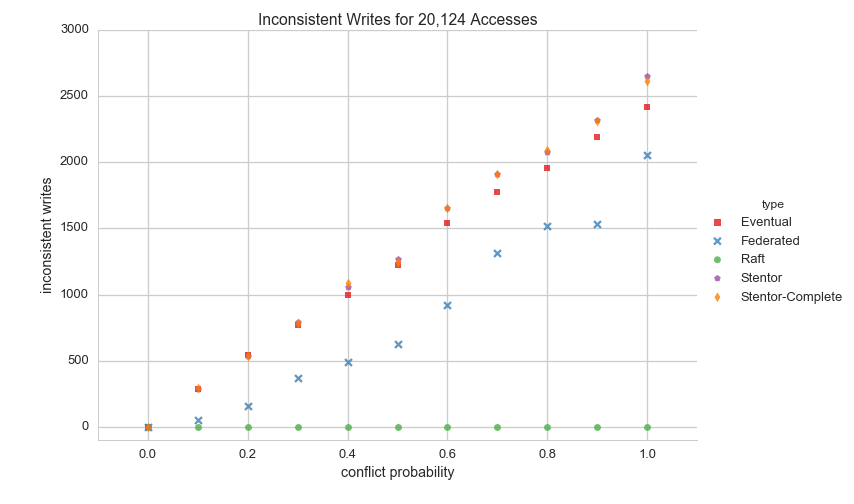
\includegraphics[width=\textwidth]{figures/inconsistent_writes.png}
        \caption{\textsf{An inconsistent write occurs when a fork gets written into the log of a node. All Eventual variations allow this and therefore have as many inconsistencies as they do forks (as shown in Figure \ref{fig:forked_writes}). Raft does not allow forked writes into the log and therefore has zero inconsistent writes. Note that although there is a linear increase in the number of forks as the conflict probability increases, most systems are able to minimize the raw number of forks to a small percentage of the total writes.\\
\\
        Federated reduces the number of inconsistencies from eventual, though not in the linear fashion that we were hoping for. In fact, it looks possibly like an exponential curve and there is some variance around $P_{conflict}=0.6-0.9$}}. I believe there is room for improvement here, as I will discuss in the following figures.
        \label{fig:inconsistent_writes}
\end{figure}

\begin{figure}[!h]
    \centering
        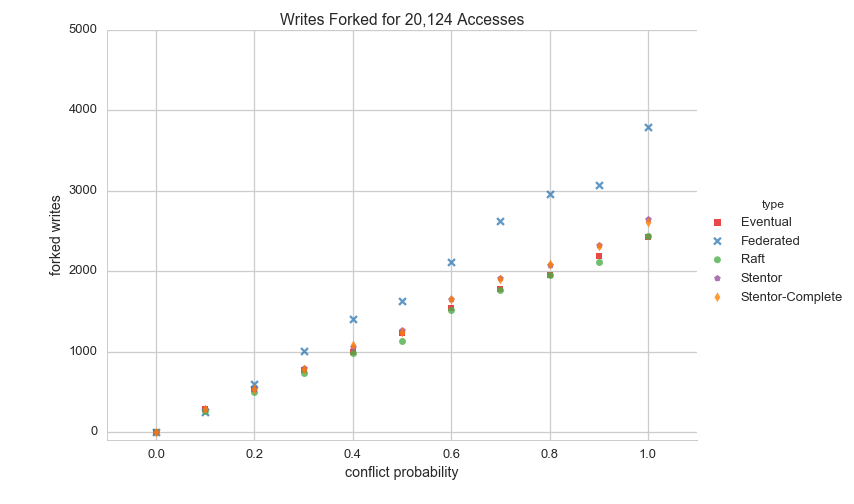
\includegraphics[width=\textwidth]{figures/forked_writes.png}
        \caption{\textsf{A forked write is a write access that follows a stale read; e.g. the local read of the object being written to is behind some global version of the object. We might also call a forked write a conflict: e.g. two nodes have concurrently written to the same object. Forked writes occur because of the delay in replicating an access across the network; the longer the potential delay the higher the possibility of a fork. \\
\\
        At first glance, this chart is disappointing, there should be less forks for Federated than other systems, and in fact my original hypothesis was that Federated reduced inconsistent and dropped writes simply by minimizing the number of Forks. However these results show that even though there are more forks, there are still less inconsistencies and drops. This might be because of the \texttt{RemoteWrite} mechanism of Federated, causing ``extra'' writes as discussed in Figure \ref{fig:committed_writes}, but these writes aren't going to be forked necessarily.\\
\\
        At second glance, however, we see that there is no real difference between the number of forks for Eventual and Raft. This implies that eventual nodes converge as fast as Raft nodes with anti-entropy as with broadcast. There are two anti-entropy sessions for every one heartbeat message given the relationship of the anti-entropy interval ($\frac {T} {4}$) and the heartbeat interval ($\frac {T} {2}$). This means a write should propagate to only 3 other nodes before an \texttt{AppendEntries} broadcast to all nodes. Therefore both Federated and Raft should have a better write propagation model and less possibility of forks.}}
        \label{fig:forked_writes}
\end{figure}


\begin{figure}[!h]
    \centering
        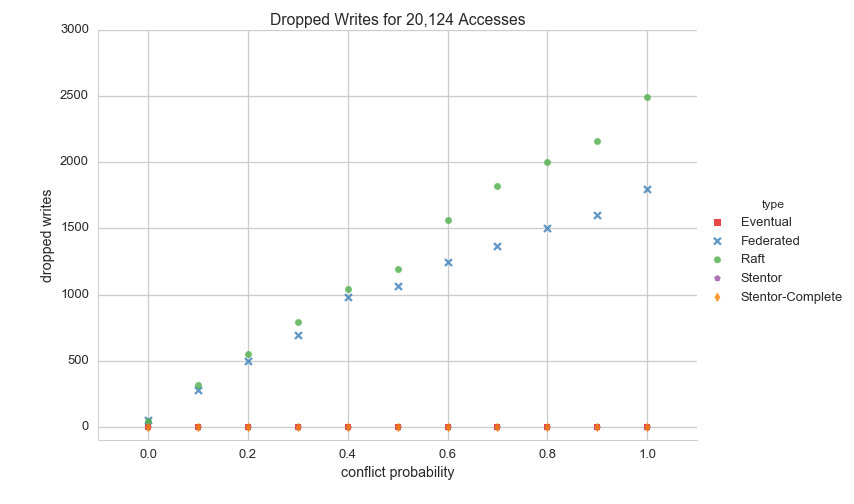
\includegraphics[width=\textwidth]{figures/dropped_writes.png}
        \caption{\textsf{When Raft encounters a fork, from a remote write, rather than writing it to the log, it drops the write and sends a failure message back to the remote writer. For Raft, the number of dropped writes is equivalent to the number of Forks. Eventual nodes do not drop writes, therefore they have zero dropped writes. Federated drops fewer writes than Raft, but again, not as many as I had hoped for via fork minimization. I believe this may have to do with Raft getting overloaded by anti-entropy writes as shown in Figure \ref{fig:committed_writes}.}}
        \label{fig:dropped_writes}
\end{figure}

\begin{figure}[!h]
    \centering
        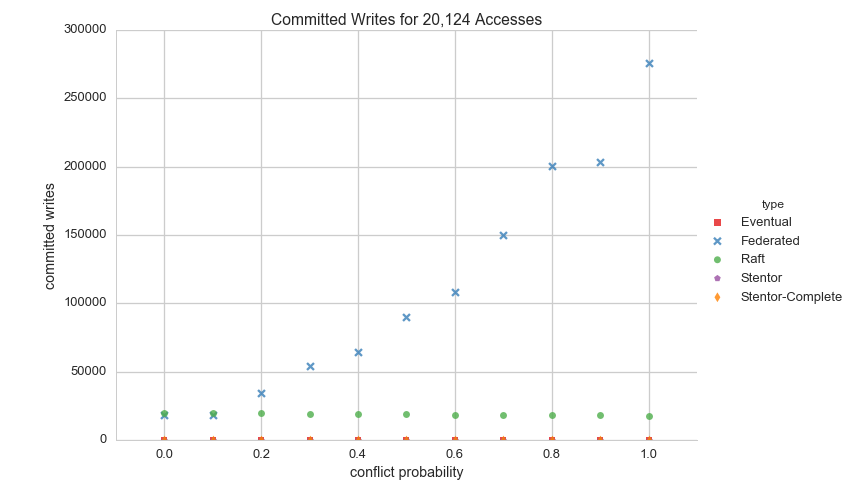
\includegraphics[width=\textwidth]{figures/committed_writes.png}
        \caption{\textsf{This figure seems to show the symptoms of Federated's problem with the eventual cloud; namely an exponential increase in the number of committed writes as conflict goes up. So how is Federated committing 14 times the number of writes as there were accesses? The issue is that Federated Raft treats anti-entropy as a remote write so long as the receiving Raft's log is earlier than object version being synchronized. Since there is the possibility of at least 2 anti-entropy sessions between every \texttt{AppendEntries} there will be a duplication of the write even if the object doesn't change because anti-entropy is sending the entire object version vector.\\
\\
        Therefore the issue seems to stem from the combination of object vector gossip plus aggregated append-entries. We may have to extend the Raft local cache to include anti-entropy writes or create a secondary cache for maintaining anti-entropy convergence.}}
        \label{fig:committed_writes}
\end{figure}

\begin{figure}[!h]
    \centering
        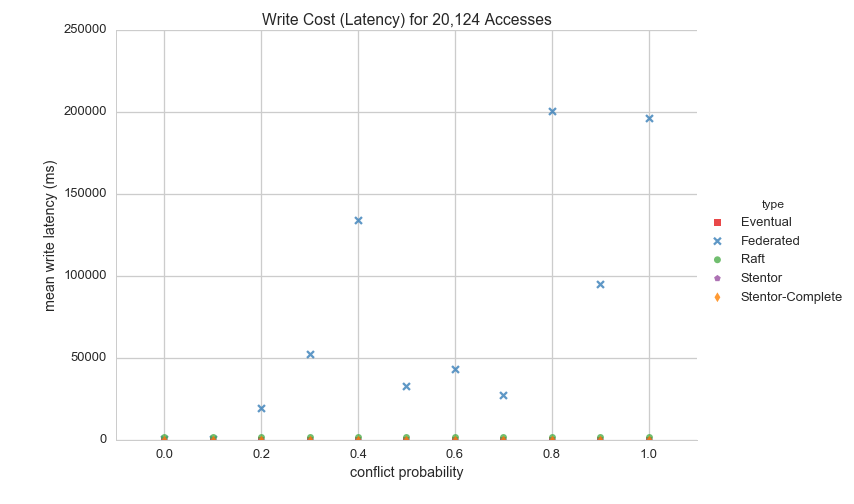
\includegraphics[width=\textwidth]{figures/write_latency.png}
        \caption{\textsf{In Federated and Raft, the write latency is measured as the delay of a \texttt{RemoteWrite}, since there are huge numbers of commits due to duplicated \texttt{RemoteWrites}, the scale of this graph only shows the extreme performance of Federated nodes.}}
        \label{fig:write_latency}
\end{figure}

\begin{figure}[!h]
    \centering
        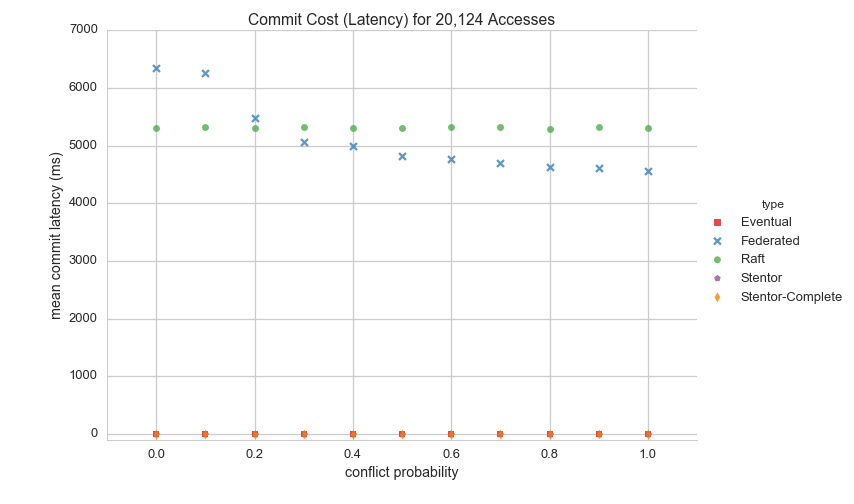
\includegraphics[width=\textwidth]{figures/commit_latency.png}
        \caption{\textsf{Commit latency measures the time from initiation of the access until it is committed by the leader. However, commit latency is only measured once (the first commit) so the duplicate commits by reissuing the write as a remote write do not appear in this graph. Note that this is not a similar case for Write latency because eventual nodes do not have the notion of a commit.}}
        \label{fig:commit_latency}
\end{figure}

\begin{figure}[!h]
    \centering
        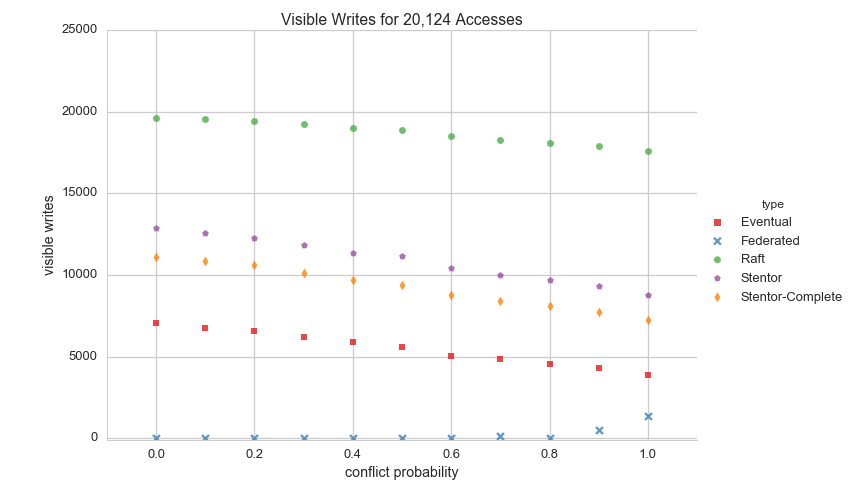
\includegraphics[width=\textwidth]{figures/visible_writes.png}
        \caption{\textsf{This metric has not been updated at the time of these simulations, so visible writes here refers to the number of fully visible writes on all replicas. Federated has typically performed very well in visibility in our previous simulations, I believe that the zero visibility may come from Federated Raft nodes not participating in anti-entropy; though it should be taken care of by synchronization to the local Raft nodes from the remotes. Potentially this has to do with the duplication of remote writes again.\\
\\
        It is useful however to look at the comparison of Stentor, Stentor-Complete, and Eventual in terms of visibility. Eventual has more visibility thanks to the object version vector than it did before, and stentor-complete has roughly double the visibility since it performs anti-entropy with 2 nodes per anti-entropy session. However, the Stentor core group actually does a better job with visibility by only allowing a subset of the nodes to move versions across the wide area! This does show there is a slight advantage to the spanning tree core, though not one that can compete with the broadcast mechanism of Raft.}}
        \label{fig:visible_writes}
\end{figure}

\begin{figure}[!h]
    \centering
        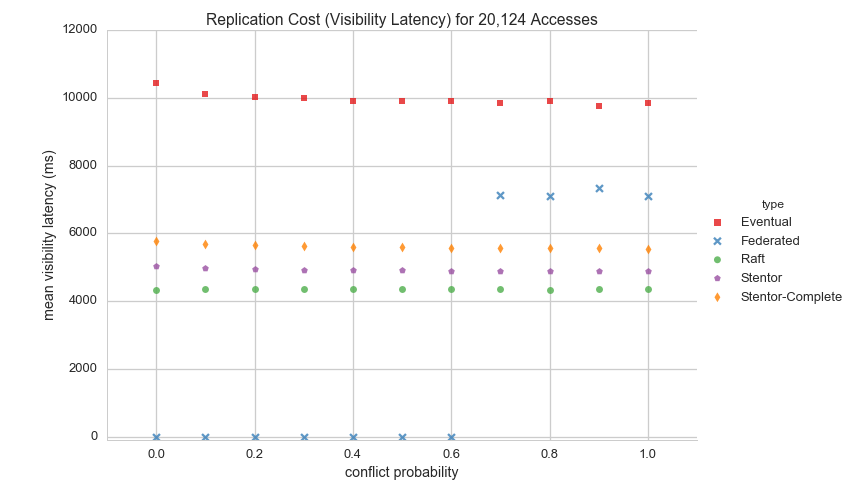
\includegraphics[width=\textwidth]{figures/visibility_latency.png}
        \caption{\textsf{Visibility latency is the time it takes for a write to become fully visible (though we will have to discuss what this metric means with the new visibility percentage metric). Raft's average visibility latency is a tad less than the heartbeat interval to account for writes that originate at the leader. Eventual has the highest delay, and stentor complete is roughly half of that delay, but again the Stentor core group performs better to stentor, and close to Raft. Since Federated isn't getting full visibility, these numbers are meaningless for it.}}
        \label{fig:visibility_latency}
\end{figure}

\begin{figure}[!h]
    \centering
        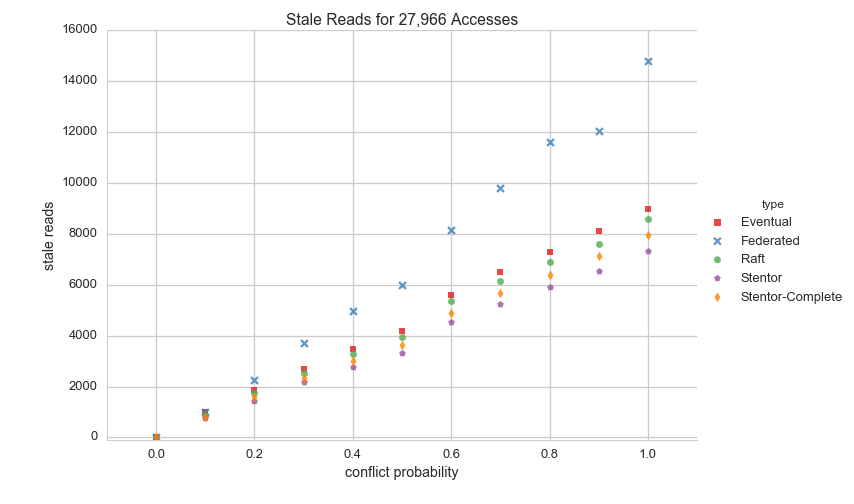
\includegraphics[width=\textwidth]{figures/stale_reads.png}
        \caption{\textsf{A stale read is a local read such that there is a global version of the object that is newer than the local read. Stale reads before writes cause forks. This graph is therefore very similar to Figure \ref{fig:forked_writes}.}}
        \label{fig:stale_reads}
\end{figure}

\begin{figure}[!h]
    \centering
        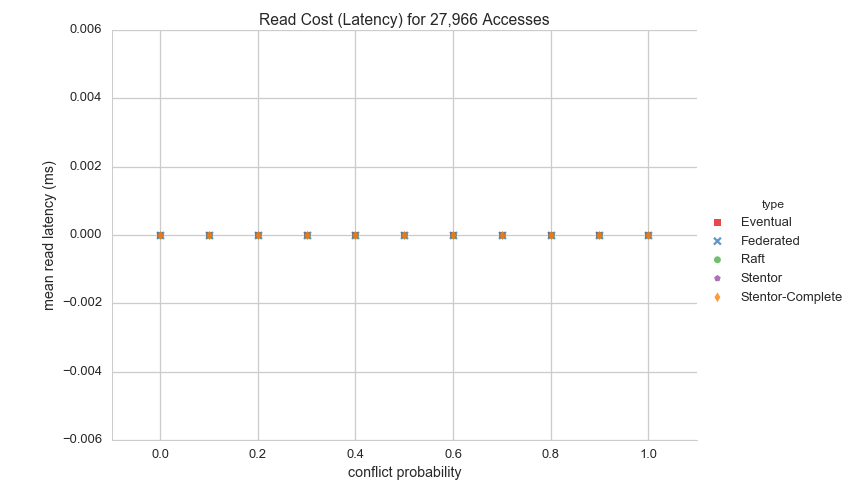
\includegraphics[width=\textwidth]{figures/read_latency.png}
        \caption{\textsf{Every node implements read local cache, therefore every node has zero read latency.}}
        \label{fig:read_latency}
\end{figure}

\begin{figure}[!h]
    \centering
        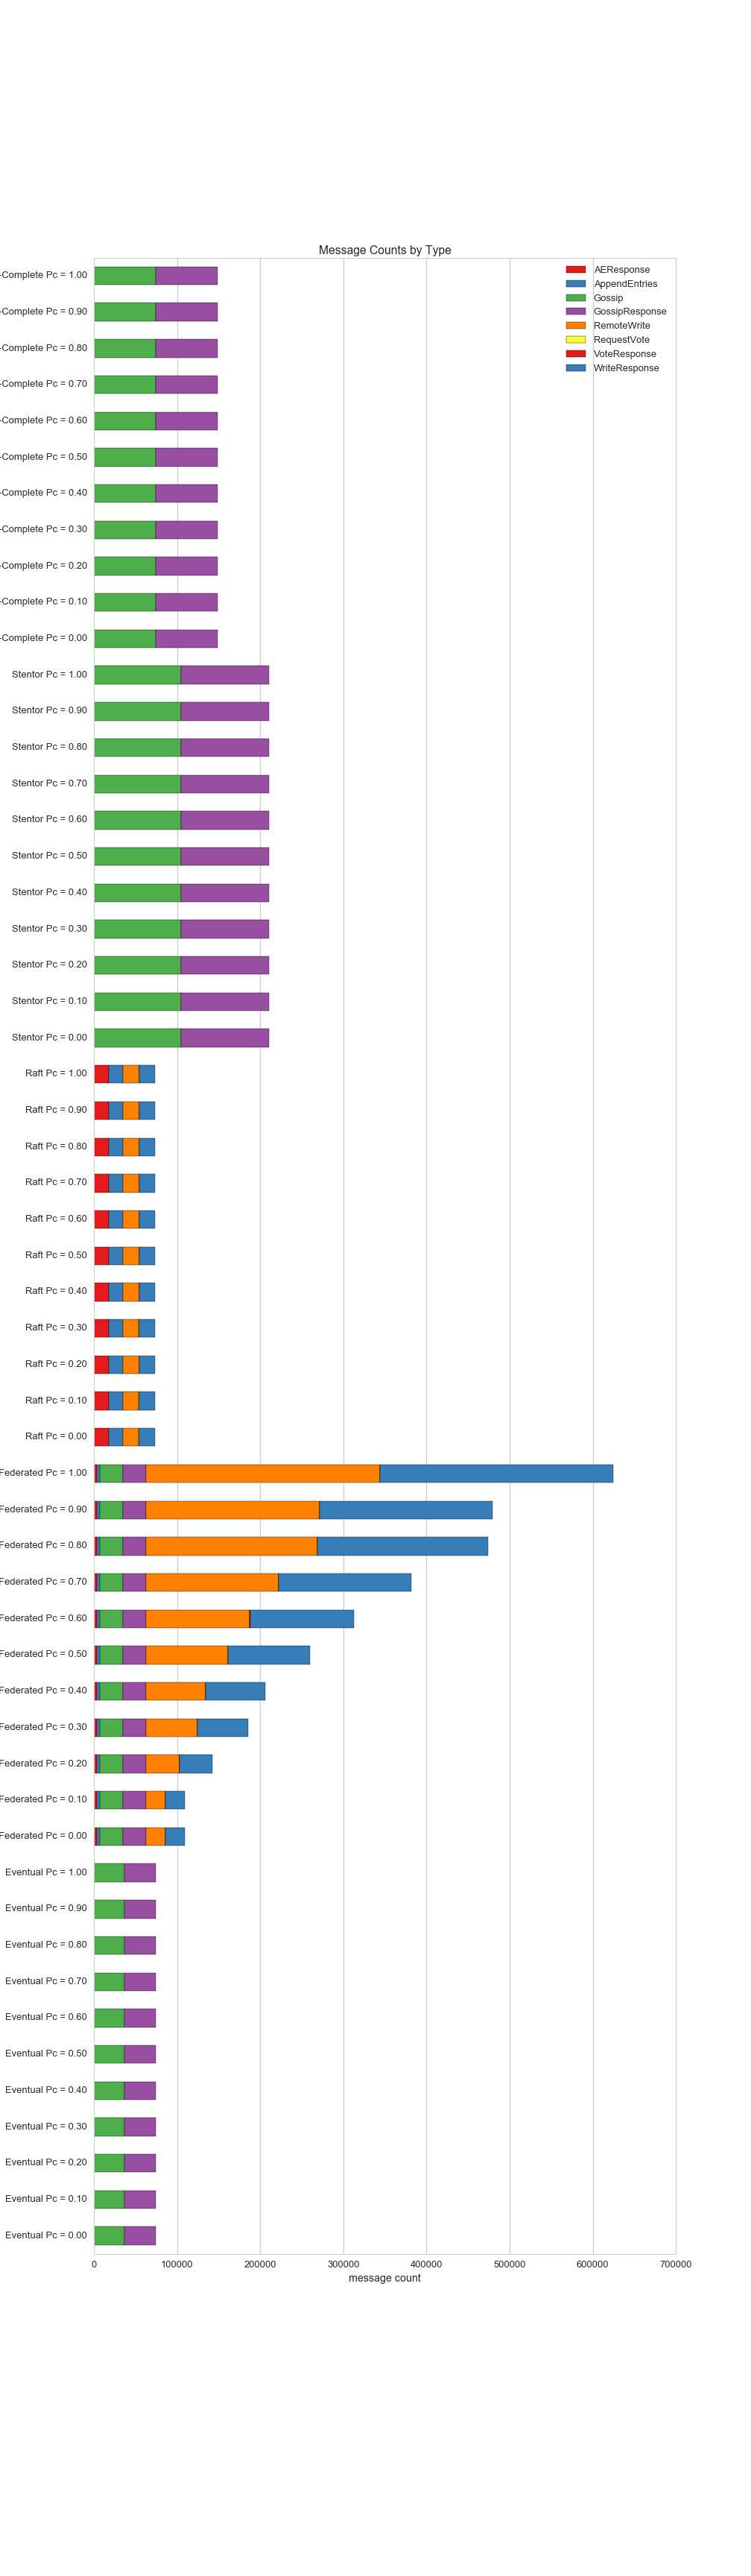
\includegraphics[height=.9\textheight]{figures/message_counts.png}
        \caption{\textsf{See \ref{fig:messages_sent} for more details.}}
        \label{fig:message_counts}
\end{figure}

\begin{figure}[!h]
    \centering
        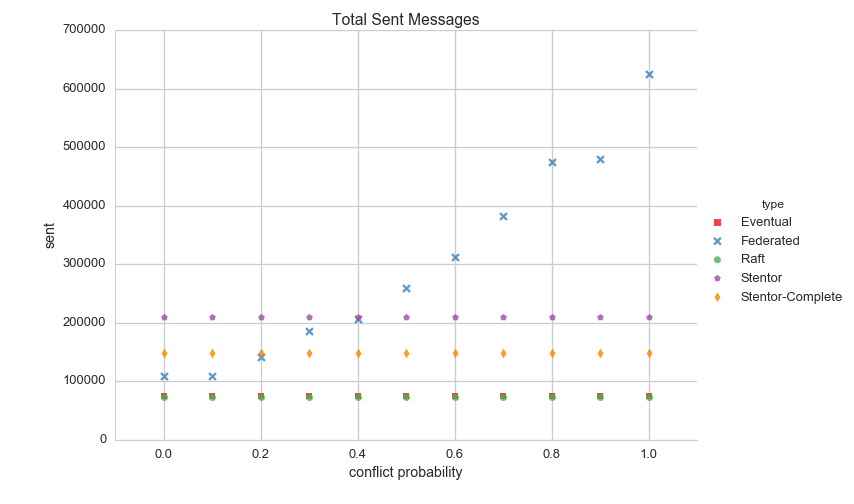
\includegraphics[width=\textwidth]{figures/messages_sent.png}
        \caption{\textsf{Raft and Eventual nodes all send the same amount of messages no matter the conflict probability because messages do not depend on conflicts. However, the Federated nodes send exponentially more messages in the form of remote writes and write responses. This was a surprise at first to me because there are more objects at the lower conflict levels (e.g. to maintain 30 objects per replica for 20 replicas at 0 conflict requires 600 distinct objects, whereas there are only 30 objects for 100\% conflict.) Therefore it seemed that there would be more remote writes due to the duplication of the remote write between append entries.\\
\\
        This graph suggests that the same effect is happening, just that the Federated Raft node is more likely to not have the later version of the object from both directions (local anti-entropy and \texttt{AppendEntries}) when conflict occurs, thus the \texttt{RemoteWrite} duplication happens at more than one FederatedRaft node, the more nodes it occurs at, the more messages are sent, therefore the exponential increase in the number of messages sent.}}
        \label{fig:messages_sent}
\end{figure}

\begin{figure}[!h]
    \centering
        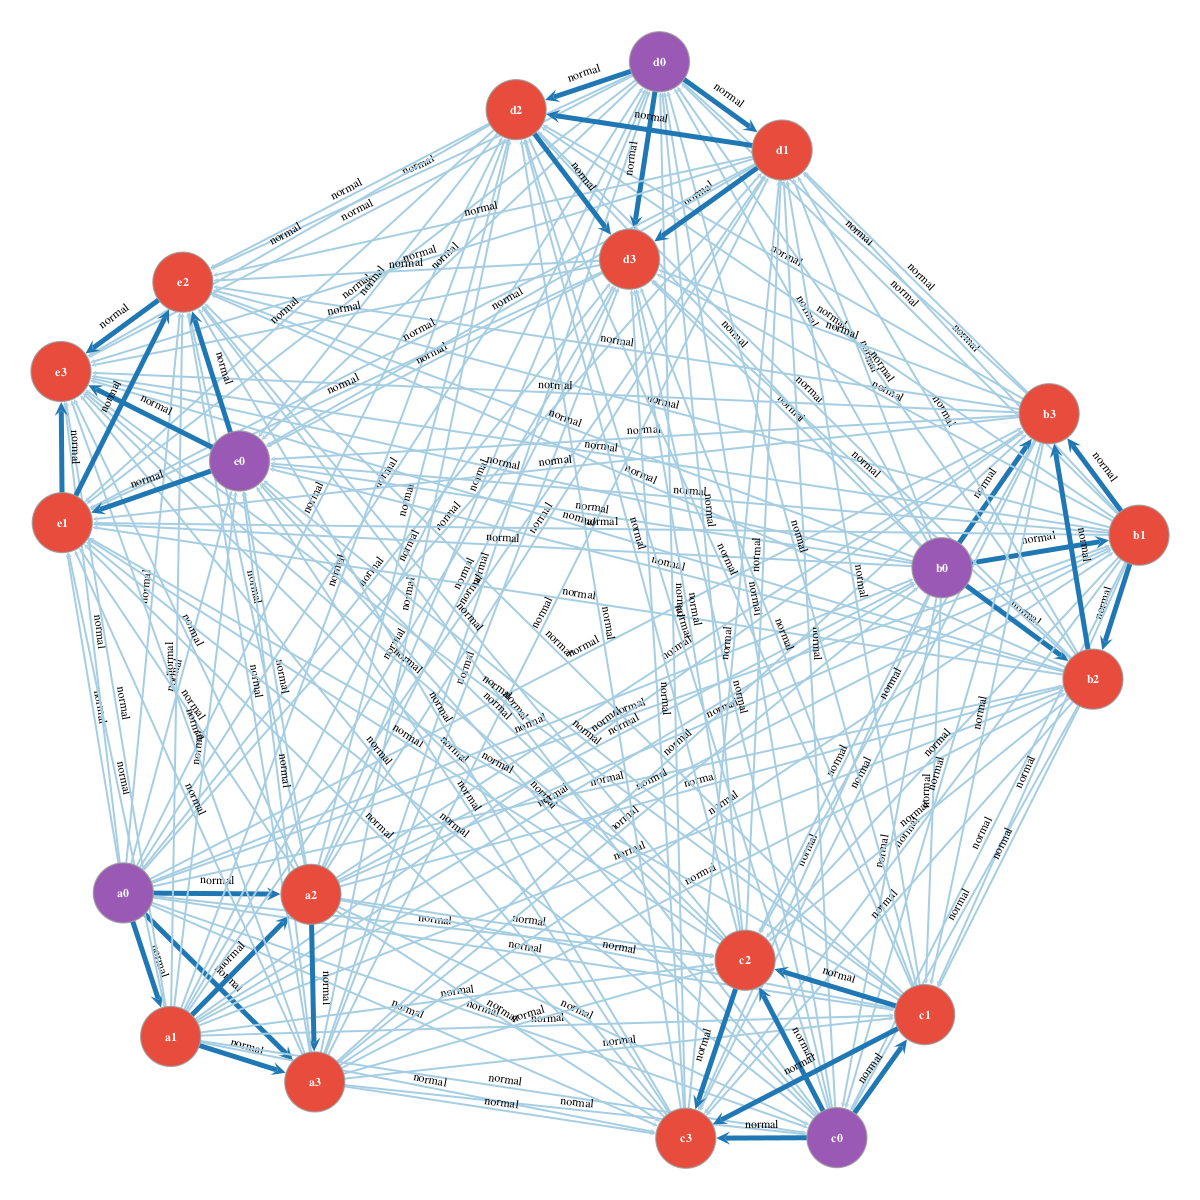
\includegraphics[width=\textwidth]{figures/stentor-topology.png}
        \caption{\textsf{This graph shows the Stentor topology, though unfortunately without access traces. The color of the node represents the replica type (red for eventual, purple for stentor) and the size of the link indicates a lower latency. This graph shows a fully connected topology of 5 areas that have faster local connections than wide area ones and that all links have normal distributions of message latency.}}
        \label{fig:topology}
\end{figure}

\begin{figure}[!h]
    \centering
        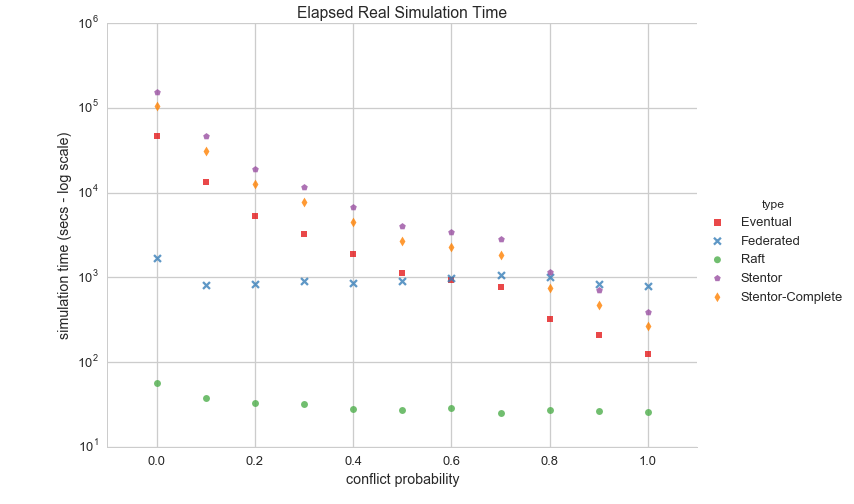
\includegraphics[width=\textwidth]{figures/simulation_time.png}
        \caption{\textsf{This graph shows the performance of the simulations in real computational time. Since simulation times are getting longer (even with high performance machines), I want to ensure that we do not bottleneck the research process, so I've started to track it.\\
\\
        I had thought that simulation time was solely dependent on the number of messages sent and their interval (thus reducing the amount of time skipped in a discrete event simulation). However, there also appears to be a relationship to the ``size'' of the message or at least the amount of processing required. Eventual, Stentor, and Stentor-Complete all perform faster with fewer objects, though they all send the same number of messages as shown in Figure \ref{fig:messages_sent}. Interestingly, Federated stays the same (approximately) even though it's sending exponentially more messages, but that's because the messages are all sent in the same time step.\\
\\
        Note that the y-axis is a log scale, therefore the linear trend lines indicate a exponential decrease.}}
        \label{fig:simulation_time}
\end{figure}

\end{document}
